%% LyX 2.0.4 created this file.  For more info, see http://www.lyx.org/.
%% Do not edit unless you really know what you are doing.
\documentclass[12pt,oneside,english]{amsart}
\usepackage[T1]{fontenc}
\usepackage[latin9]{inputenc}
\usepackage{geometry}
\geometry{verbose,lmargin=1.25in,rmargin=1.25in}
\usepackage{amsthm}
\usepackage{tikz}
\usepackage{array}
\usetikzlibrary{arrows}


\makeatletter
%%%%%%%%%%%%%%%%%%%%%%%%%%%%%% Textclass specific LaTeX commands.
\numberwithin{equation}{section}
\numberwithin{figure}{section}
\theoremstyle{plain}
\newtheorem{thm}{\protect\theoremname}
  \theoremstyle{definition}
  \newtheorem{defn}[thm]{\protect\definitionname}
  \theoremstyle{plain}
  \newtheorem{lem}[thm]{\protect\lemmaname}

\makeatother

\usepackage{babel}
  \providecommand{\definitionname}{Definition}
  \providecommand{\lemmaname}{Lemma}
\providecommand{\theoremname}{Theorem}

\begin{document}

\section{Introduction}


\subsection{Organization of the Report}


\subsection{Preliminaries}

We will begin by formalizing the classic online bipartite matching
problem and providing definitions of some terms which we will use
throughout this paper.


\subsubsection{Classic Online Bipartite Matching Problem Definition}

In the classic version of the problem, we define the input as the
bipartite graph $G=(U,V,E)$, where $U$ and $V$ are two independent
sets of $n$ vertices each and $E$ is the set of edges connecting
the vertices in $U$ to the vertices in $V$. For this problem we
assume that our algorithm has full access to all of the vertices in
$V$ from the beginning, but receives each vertex $u\in U$ one at
a time in a preselected order. Each time a vertex $u\in U$ is received,
the edges incident to $u$ become known to the algorithm and the algorithm
is thus tasked with permanently matching $u$ to an adjacent, unmatched
vertex $v\in V$ if possible. The goal of the problem is t o create
the largest sized matching possible. Unless otherwise stated, we assume
that $G$ has a perfect matching and thus the size of the optimal
matching is $n$.


\subsubsection{Useful Definitions}
\begin{defn}
We let $N(u)\subset V$ to be the set of previously unmatched vertices
in $V$ that are adjacent to a vertex $u\in U$.
\end{defn}
Thus, it is not until the algorithm receives a vertex $u\in U$ that
the set of vertices $N(u)$ becomes known.
\begin{defn}
We define $m$ as the algorithms current matching and $m(u)$ as the
vertex $v\in V$ that $u$ is matched with. Furthermore, we define
$m^{*}$ as an optimal matching, which we assume is a perfect matching.
\end{defn}

\section{Classic Online Bipartite Matching Algorithms}

Below we present and analyze two algorithms for the classic online
bipartite matching problem: the Greedy algorithm and the Ranking algorithm.


\subsection{Greedy Algorithm}

The Greedy algorithm, despite its simplicity and na�vet�, actually
provides a reasonable competitiveness, which, as we will later prove,
is optimal for deternministic algorithms.


\subsubsection{Greedy Algorithm Description}

As one might expect, upon reception of a vertex $u\in U$ the Greedy
algorithm always, simply matches $u$ with an arbitrary vertex $v\in N(u)$
if $N(u)\ne\emptyset$. 


\subsubsection{Greedy Algorithm Analysis}

It is easy to see that the Greedy algorithm has a competitive ratio
of at least $\frac{1}{2}$, because for every vertex $u$ it is either
the case that $u$ is matched to some vertex $v\in V$ or $N(u)=\emptyset$.
Remember, we assume that there exists a perfect matching $m^{*}$
which matches all $2n$ of the vertices in $n$ matchings. For every
vertex $u\in U$, at least one of $u$ or $m^{*}(u)$ must be in our
Greedy algorithm's matching. Thus, our algorithm matches a minimum
of $n$ vertices in total in a minimum of $\frac{n}{2}$ matchings. 


\subsubsection{Greedy Algorithm Optimality}

We can further demonstrate that no deterministic algorithm can have
better competitiveness than $\frac{1}{2}$. Suppose, for example,
an adversarial input in which each of the first $\frac{n}{2}$ vertices
from $U$ that the algorithm receives are adjacent to every vertex
$V$. Then the remaining $\frac{n}{2}$ vertices from U are only adjacent
to the vertices that the algorithm was determined to have already
matched. Thus, clearly for every deterministic algorithm there is
an input for which it is $\frac{1}{2}$ competitive.


\subsection{Ranking Algorithm}

Since the upperbound for the competitiveness of determinstic algorithms
is $\frac{1}{2}$, we will need to add randomization in order to get
an improvement. Luckily, by simply adding a single element of randomness
and tweaking our Greedy algorithm so that there is no arbitrary choice,
we can get an improved expected competitiveness. 


\subsubsection{Ranking Algorithm Description}

The Ranking algorithm begins with an initialization phase that consists
of choosing a random permutation of the vertices in $V$, which will
serve as the basis for our ranking function $\sigma$. Then upon receiving
each vertex $u\in U$, the algorithm matches $u$ to the vertex $v\in N(u)$
which minimizes $\sigma(v)$, such that $v$ has not already been
matched. Obviously, if every vertex adjacent to $u$ is already matched,
i.e. $N(u)=\emptyset$, the algorithm does not match $u$.


\subsubsection{Ranking Algorithm Analysis}

Like in the Greedy algorithm, a received vertex $u\in U$ is not matched
if and only if $N(u)=\emptyset$. As a result, we know that its competitiveness
is always at least $\frac{1}{2}$. Since, the Ranking algorithm has
a random element to it, it is not bounded in the same way that deterministic
algorithms are, which leads us to the following theorem.
\begin{thm}
The Ranking algorithm has an expected competitiveness of $1-\frac{1}{e}\approx0.63$.
\end{thm}
We will ``prove'' this theorem with an extremely intuitive, but
slightly incorrect proof. We encourage enthusiastic readers to read
{[}{[}{[}{]}{]}{]}, if they would like to get the correct, but more
technical version of the proof.

Let us define $m_{\sigma}$ as the matching produced by the Ranking
algorithm with ranking function $\sigma$ for some given input. We
can relate Ranking($\sigma$) with the optimal matching $m^{*}$ using
the following lemma.
\begin{lem}
\label{lem:For-every-vertex}For every vertex $u\in U$, if vertex
$v=m^{*}(u)$ is not matched in $m_{\sigma}$, then in $m_{\sigma}$
$u$ is matched to a vertex $v'=m_{\sigma}(u)$ such that $\sigma(v')<\sigma(v)$.\end{lem}
\begin{proof}
Since vertex $v$ is not matched in $m_{\sigma}$, that means that
when $u$ was recieved by the Ranking algorithm, $v$ was still unmatched.
Thus, the only reason $u$ would not be matched to $v$ would be if
it could get matched to a higher ranking vertex $v'$, such that $\sigma(v')<\sigma(v)$.
\end{proof}
We will use the following lemma to get our competitiveness.
\begin{lem}
\label{lem:If-we-define}If we define $x_{t}$ as the probability
over ranking function $\sigma$ that the vertex $v\in V$ such that
$\sigma(v)=t$ is matched in $m_{\sigma}$, then $1-x_{t}\le\frac{1}{n}\underset{1\le s\le t}{\sum}x_{s}$
for all $t$ in range $[1,n]$.\end{lem}
\begin{proof}
Let us define $u$ as the vertex in $U$ that $v$ is matched with
in the optimal matching, i.e. such that $v=m^{*}(u)$. Furthermore,
let us define the set of vertices $R_{t-1}\subset U$ as the set of
vertices in $U$ that are matched in $m_{\sigma}$ to vertices in
$V$ of rank that is no more than $t-1$. In otherwords for all $u\in U$
such that $u$ is matched in $m_{\sigma}$, $u$ is in $R_{t}$ if
and only if $\sigma(m_{\sigma}(u))<t$. By Lemma \ref{lem:For-every-vertex},
if vertex $v$ is not matched in $m_{\sigma}$, then $u\in R_{t}$.
Thus, the probability that $v$ is not matched in $m_{\sigma}$ is
bounded by the probability that $u\in R_{t}$. Clearly, by the defintion
of $x_{t}$, the probability that $v$ is not matched is $1-x_{t}$
and the expected size of $R_{t}=\underset{1\le s<t}{\sum}x_{s}$.
If $u$ and $R_{t}$ were independent, then the probability that $u\in R_{t}$
would simply be $\frac{|R_{t}|}{n}=\frac{1}{n}\underset{1\le s<t}{\sum}x_{s}$,
which would complete our lemma with $1-x_{t}\le\frac{1}{n}\underset{1\le s<t}{\sum}x_{s}\le\frac{1}{n}\underset{1\le s\le t}{\sum}x_{s}$
.

However, this is where this proof fails. The fact is $u$ and $R_{t}$
are not actually independent in the way we set it up. The correct,
but less intuitive, proof demonstrates how choosing vertices $v$
and $u$ randomly and independently of $\sigma$ can result in having
the relation that if vertex $v$ is not matched in $m_{\sigma}$,
then $u\in R_{t+1}$. In this case $u$ and $R_{t+1}$ are independent,
which correctly proves the lemma. Again, we encourage interested readers
to read the correct proof in {[}{[}{[}{]}{]}{]}{]}.
\end{proof}
Now we can compute the expected competetiveness. It is easy to see
that the expected size of $m_{\sigma}$ is $\sum_{1\le s\le t}x_{s}$.
Since we are assuming that there exists a perfect matching, that means
the expected competitiveness is $\frac{1}{n}\sum_{1\le s\le n}x_{s}$,
which we must lower bound using Lemma \ref{lem:If-we-define}. If
we define $S_{t}=\sum_{1\le s\le t}x_{s}$, we can rewrite Lemma \ref{lem:If-we-define}
to $1-(S_{t}-S_{t-1})\le\frac{1}{n}S_{t}$, which can be simplified
to $1+S_{t-1}\le\left(\frac{n+1}{n}\right)S_{t}$. It follows that
$S_{t}$, and by extension also $\frac{1}{n}\sum_{1\le s\le t}x_{s}$,
is smallest when all of the inequalites are equalities, which gives
us $S_{t}=\sum_{1\le s\le t}\left(\frac{n}{n+1}\right)^{s}$. As a
result, our expected competitiveness $\frac{1}{n}\sum_{1\le s\le n}x_{s}=\frac{S_{n}}{n}$
is lower bounded by $\frac{1}{n}\sum_{1\le s\le n}\left(\frac{n}{n+1}\right)^{s}$
which after some mathemagic becomes $1-(\frac{n}{n+1})^{n}$ which
approaches $1-\frac{1}{e}$ as $n$ goes to infinity, thus concluding
our proof.


\subsubsection{Optimality of Ranking Algorithm}

\section{Online Vertex-Weighted Bipartite Matching}

The online vertex-weighted bipartite matching problem is a generalization of the online bipartite matching problem. The difference is that each vertex in $V$ now has an associated weight. Instead of maximizing the size of the matching, we now aim to maximize the total weight of the vertex of $V$ which are included in the matching. The online bipartite matching problem described in Section ?? is the special case where all edges in $V$ have weight 1.

Formally, the input to the problem is a bipartite graph $G = (U, V, E, \{w_v\}_{v \in V})$. The vertices in $V$ as well as their weights are known ahead of time. The vertices in $U$ arrive online. As before, the edges of a vertex $u \in U$ are revealed when $u$ arrives. When a vertex arrives it can either be matched to a neighbor in $V$ or not matched. However, once made, a decision cannot be undone. We aim to maximize the sum of weights of all the matched vertices in $V$. As before, we will assume that $|U| = |V|$ and that $G$ contains a perfect matching.

\subsection{Greedy Algorithm}

The obvious greedy solution to this problem is to match a vertex $u \in U$ to its neighbor of greatest weight, or leave it unmatched if it has no remaining neighbors. Call this algorithm $\textsc{Greedy}$.

\begin{lem}
\textsc{Greedy} is a (1/2)-approximation for vertex-weighted bipartite matching. Furthermore, this is the best approximation ratio the algorithm can achieve.
\end{lem}

\begin{proof}
First we show that \textsc{Greedy} is a (1/2)-approximation. Let $O \subseteq E$ be the optimal offline matching, and $A \subseteq E$ be the matching produced by $\textsc{Greedy}$. If $A \neq O$, then there is some $v_{O} \in V$ such that $v_{O}$ is in $O$ but not $A$. Let $u$ be the vertex which was matched to $v_{O}$ in $O$. Then there must be some other vertex $v_{A}$ such that $u$ was matched to $v_{A}$ in $A$. This is because we know that $v_O$ was unmatched when $u$ was being matched, so the only way $u$ would not be matched to $v_O$ is if there were some other neighbor with greater weight.

But now we have that the optimal value `lost' by $u$ is at most equal to the weight of its match in $A$. Therefore the total amount which $|A|$ losses is $A$. Hence, $|A| \geq |O|/2$.

To see that this is the tightest approximation ratio for this algorithm, we offer an example. Consider the following graph.

\begin{center}
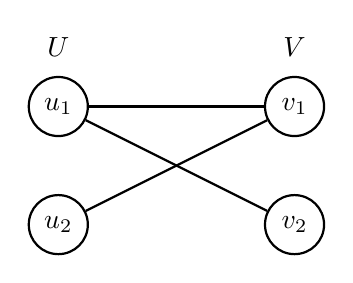
\begin{tikzpicture}[-,>=stealth',auto,
  thick,main node/.style={circle,draw, minimum size = 0.75cm}]

\node[draw = white] (a) at (0, 2.25){$U$};
\node[draw = white] (b) at (3, 2.25){$V$};

\node[main node] (v) at (0, 1.5){$u_1$};
\node[main node] (w) at (0, 0){$u_2$};

\node[main node] (v1) at (3, 1.5){$v_1$};
\node[main node] (w1) at (3, 0){$v_2$};

\path[]


(w) edge node [below] {} (v1)
(v) edge node [below] {} (w1)
(v) edge node [below] {} (v1);

\end{tikzpicture}
\end{center}

Let $w_{v_1} = 1 + \epsilon$ for some $\epsilon > 0$ and $w_{v_2} = 1$. Then the greedy algorithm will match only $(u_1, v_1)$, and the optimal solution will match $(u_1, v_2), (u_2, v_1)$. As $\epsilon$ approaches 0, the approximation ratio approaches $1/2$.

\end{proof}

We will not offer a proof here, but it turns out that no deterministic algorithm can do better than $\textsc{Greedy}$.

\subsection{Generalizing Ranking}

Consider the \textsc{Ranking} algorithm described above. For an input in which the range of weights is small, this algorithm will perform well. This is reflected in the fact that \textsc{Ranking} is optimal in the case where all weights are equal. However, when the range of weights is large, this algorithm can perform very poorly.

We want to generalize the ranking algorithm in order to account for the weighted case. We will present a new algorithm which we will call \textsc{Perturbed-Greedy}. We will show that this algorithm is equivalent to \textsc{Ranking} in the case where all weights are equal, and we will show that this algorithm achieves an approximation ratio of $1 - \frac{1}{e}$.

The \textsc{Perturned-Greedy} algorithm will use the function
\[\psi(x) = 1 - e^{x - 1}.\]

\begin{enumerate}
\item For each $v \in V$, choose $x$ uniformly at random from $[0, 1]$.
\item For arriving $u \in U$, match $u$ to the unmatched neighbor $v$ with highest value $b_v\psi(x)$.
\item Break ties by vertex ID.
\end{enumerate}

Consider the case where all weights are equal. Since $x$ is chosen uniformly at random, choosing vertices according to the highest values of $b_v\psi(x)$ is equivalent to choosing a random ranking. Thus, \textsc{Perturbed-Greedy} is equivalent to \textsc{Ranking} when all weights are equal, as desired.

We will prove the following Theorem.

\begin{thm}
\text{Perturned-Greedy} achieves an approximation ratio of $1 - \frac{1}{e}$ for the vertex-weighted online bipartite matching problem.
\end{thm}

While we will not offer a proof here, it turns out that this is the optimal approximation ratio for this problem. Intuitively, this result seems reasonable because we know that this is the optimal approximation ratio for a more specific version of this problem.

\begin{proof}
Proof here.
\end{proof}


\end{document}
